% Auto-generated by scripts/make_figures.py from
% outputs/design_exercise/rule_comparison.csv. Do not edit by hand.

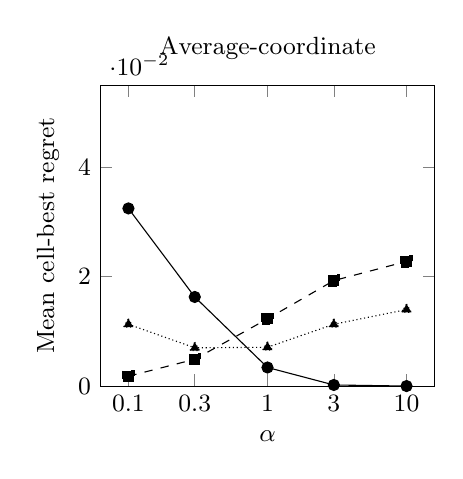
\begin{tikzpicture}
\begin{axis}[
  width=0.48\textwidth, height=5.4cm,
  xmode=log, log ticks with fixed point,
  xtick={0.1,0.3,1,3,10}, xticklabels={0.1,0.3,1,3,10},
  xlabel={$\alpha$}, ylabel={Mean cell-best regret},
  ymin=0, ymax=0.055,
  title={\small Average-coordinate}, label style={font=\small},
  tick label style={font=\small},
  legend to name=leg:regret,
  legend columns=3, legend style={font=\small, /tikz/every even column/.append style={column sep=0.4cm}},
]
\addplot[solid, mark=*] coordinates {(0.1,0.0325) (0.3,0.0163) (1,0.0034) (3,0.0002) (10,0.0000)};
\addlegendentry{Frequency guessing}
\addplot[dashed, mark=square*] coordinates {(0.1,0.0018) (0.3,0.0049) (1,0.0123) (3,0.0193) (10,0.0228)};
\addlegendentry{Squared distance}
\addplot[densely dotted, mark=triangle*] coordinates {(0.1,0.0113) (0.3,0.0070) (1,0.0071) (3,0.0113) (10,0.0140)};
\addlegendentry{Manhattan distance}
\end{axis}
\end{tikzpicture}
\hfill
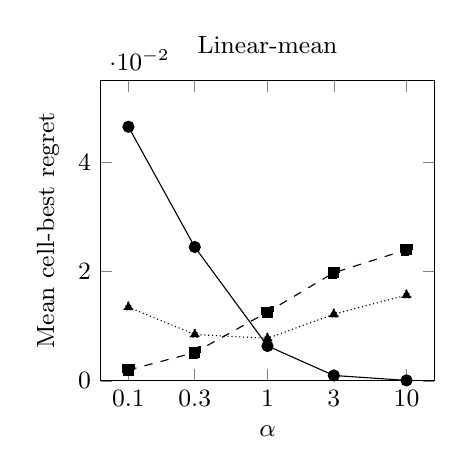
\begin{tikzpicture}
\begin{axis}[
  width=0.48\textwidth, height=5.4cm,
  xmode=log, log ticks with fixed point,
  xtick={0.1,0.3,1,3,10}, xticklabels={0.1,0.3,1,3,10},
  xlabel={$\alpha$}, ylabel={Mean cell-best regret},
  ymin=0, ymax=0.055,
  title={\small Linear-mean}, label style={font=\small},
  tick label style={font=\small},
]
\addplot[solid, mark=*] coordinates {(0.1,0.0465) (0.3,0.0245) (1,0.0064) (3,0.0010) (10,0.0001)};
\addplot[dashed, mark=square*] coordinates {(0.1,0.0020) (0.3,0.0052) (1,0.0126) (3,0.0198) (10,0.0240)};
\addplot[densely dotted, mark=triangle*] coordinates {(0.1,0.0135) (0.3,0.0085) (1,0.0078) (3,0.0122) (10,0.0157)};
\end{axis}
\end{tikzpicture}
\par\smallskip\centerline{\pgfplotslegendfromname{leg:regret}}
